\chapter{Evaluation und Validation}
\label{ch:evaluation}

% Auswertung und Interpretation der Ergebnisse. Nachweis, dass die Ziele erreicht wurden, oder
% warum welche nicht erreicht wurden.

In diesem Kapitel werden nun die Ergebnisse dieser Arbeit ausgewertet.
Im ersten Abschnitt \fullref{sec:messresultate} werden die Messungen
ausgewertet und die Messresultate graphisch illustriert und interpretiert.
Anschliessend wird im Abschnitt \fullref{sec:vergleich_anforderungen} überprüft inwiefern die Projektanforderungen erfüllt werden konnten.
Daraufhin werden im Abschnitt~\fullref{sec:technische_aspekte} die verwendeten Tools und die Architektur evaluiert.
Zuletzt wird das Vorgehen während des Projekts beurteilt (siehe Abschnitt~\fullref{sec:eval_vorgehen}).

\section{Messresultate}\label{sec:messresultate}

Als Erstes wurde die Testumgebung dahingehend überprüft, ob sie überhaupt sinnvolle Resultate misst.
Anschliessend wurden zwei verschiedene Arten von Messungen durchgeführt.
Für weitere Messungen, vor allem für Messungen mit Bandbreitenbeschränkung, war die Zeit leider zu knapp.

Bei jeder Messung wurden 1000 Nachrichten von einem zufälligen Knoten verschickt
und von einem anderen zufälligen Knoten im Testnetzwerk wieder empfangen.
Zudem wurde die konfigurierte Tunnellänge bei jeder Messung auf dem Standardwert \lstinline|3| belassen.
Die Nachrichten wurden jeweils in einem Abstand von sechs Sekunden nacheinander verschickt,
um das Netzwerk auf keinen Fall zu überlasten.
Zudem wurde jeweils die CPU-Ressourcenauslastung und Netzwerkbelastung alle 5 Sekunden gemessen.

\subsection{Validation der Testumgebung}\label{sec:validation_testumgebung}

Um Aussagen über das Testnetzwerk und dessen Messresultate machen zu können,
muss erst sichergestellt werden, dass die Messwerte überhaupt Sinn ergeben.
Deshalb wurden erste Messungen und Tests durchgeführt, um zu prüfen, ob die Testumgebung auch richtig funktioniert.
% Um sicherzustellen, dass kein Fehler beispielsweise im implementieren Testnetzwerk oder gar in der i2pd-Software aufzufinden ist, wird diese Messung zu Validierungszwecken durchgeführt.

Als Teil dieser Messung wird erst ein Netzwerk mit 8 Knoten getestet und die Latenz von 1000 Nachrichten gemessen.
Alle Knoten haben in diesem Test keine Bandbreitenbeschränkung.
Die konfigurierte Nachrichtengrösse wurde jeweils auf 64 kB festgelegt.

Als erstes wurde die Messumgebung auf meinem Laptop (8 Kerne, Intel Core i7-8550U CPU @ 1.80 GHz, mit 16 GB RAM) getestet mit 8 Knoten und dieselbe Messung mehrfach wiederholt.
Dies hatte jeweils fast immer dasselbe Resultat zur Folge:
Die Nachrichten wurden mit einer Latenzzeit von etwas mehr als fünf Sekunden empfangen.
Einige Ausreisser waren jedoch zu beobachten;
Bei manchen Nachrichten liess sich eine Latenzzeit von etwas mehr als sechs Sekunden oder bis hin zu einem Vielfachen von fünf Sekunden beobachten.
Die Neuerstellung der Tunnels, Abfragen an der NetDb, andere Effekte wie eine kurzzeitige Überlastung oder das Scheduling des Kernels könnten eine Erklärung sein für die Ausreisser von sechs Sekunden.
Die Ausreisser bei welchen sich ein Vielfaches der Latenzzeit beobachten liess,
könnten sich durch die wiederholte Übermittlung von Nachrichten im Fehlerfall
oder einem Fehler in der \lstinline|i2pd|-Software erklären.

Anschliessend wurde eine virtuelle Maschine beim Anbieter Hetzner (16 Kerne, AMD EPYC CPU @ 2.495 GHz, mit 32 GB RAM) bestellt, um dort die Messungen durchzuführen.
Alle weiteren Messungen wurden auf dieser Maschine durchgeführt.
Dort lieferte derselbe Testaufbau auch bei wiederholten Messungen dieselben Resultate.
Die Nachrichten wurden mit einer Latenzzeit von etwas mehr als fünf Sekunden empfangen
und dieselben Ausreisser (jedoch nicht ganz so häufig) von sechs Sekunden bis hin zu einem Vielfachen von fünf Sekunden konnten beobachtet werden.
Somit ist sichergestellt, dass die Messungen wiederholbar und reproduzierbar sind und eine Basis einen Referenzpunkt für weitere Messungen bieten können.

% \subsection{Wiederholbarkeit von Messungen}
%
% Eine Nachricht wird hier jeweils von einem zufälligen Knoten an einen anderen zufälligen Knoten versendet.
% Die Konfigurierte Nachrichtengrösse wurde jeweils auf 64kB festgelegt.
% Die Messung wird so festgehalten.
% Anschliessend wird derselbe Test noch einmal gestartet, wobei das Testnetzwerk jedoch aber neu erstellt wird.
%
% Grundsätzlich wird hier erwartet, dass die Messungen vergleichbar sind und ähnliche Resultate liefern.
%
% Somit kann ausgesagt werden das die Messungen so gut wie möglich reproduzierbar sind \seereq{TREP}.


\subsection{Gleichbleibende Latenz bei Skalierung des Netzwerks}\label{sec:messung_latenz}

Um nun die Hypothese \ref{hyp:first} zu bearbeiten, wird als Erstes die Anzahl Knoten skaliert
und die Latenz mehrmals unter gleichen Bedingungen gemessen.
Die konfigurierte Nachrichtengrösse wurde jeweils auf 64 kB festgelegt.
Es wird angenommen, dass sich die Latenz der Nachrichten im Netzwerk hier nicht verändert.
Dies mag auf den ersten Anschein der Hypothese widersprechen, jedoch gilt es zu beachten, dass hier alle Knoten dieselbe Bandbreitenbeschränkung von 100000 kB/s haben.
Dementsprechend müsste die Peer-Selektion von I2P alle Knoten gleich bewerten.
Der einzige Unterschied zwischen einem kleineren Netzwerk und einem grösseren Netzwerk ist somit,
dass eine grössere Auswahl an Knoten besteht, an denen eine Nachricht weitergeleitet werden kann.
Die Anzahl Knoten in den Tunnels bleibt jedoch gleich, es kommen lediglich weniger Knoten zum Einsatz bei einem kleineren Netzwerk.
Die Erwartung ist daher, dass die Latenz bei steigender Anzahl Knoten gleich bleibt.

\begin{figure*}[htp]
  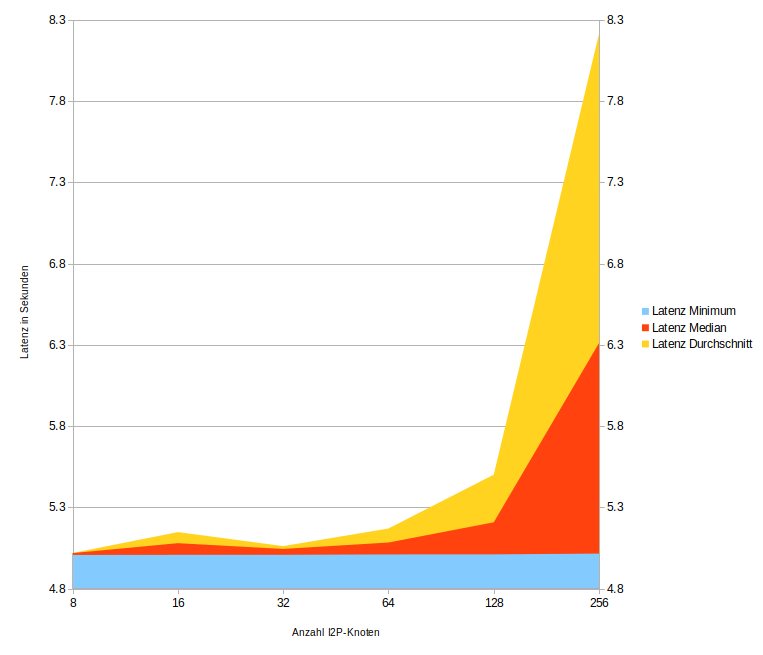
\includegraphics[width=1.1\textwidth]{img/auswertung-latenz.png}
  \caption{Nachrichtenlatenz bei Skalierung der Anzahl I2P-Knoten}\label{fig:auswertung-latenz}
\end{figure*}


Die Abbildung~\fullref{fig:auswertung-latenz} zeigt jedoch ein anderes Bild.
Während die Mindestlatenz der 1000 Nachrichten konstant auf fünf Sekunden bleibt, vergrössert sich die Median- und Durchschnittslatenz je mehr Knoten im Testnetzwerk vorhanden sind.
Vor allem bei einem Netzwerk von 256 Knoten steigt diese beträchtlich an.
Dies ist ein überraschendes Ergebnis und die Gründe sind unklar.
Es könnte sein, dass das man hier auf gewisse implizite Limits im Linux-Kernel bei dieser Menge an Docker-Containern stösst
und dass man hier auf ein Problem mit der Testinfrastruktur gestossen ist.
Jedoch ist die CPU-Auslastung im gemessenen Fünf-Sekunden-Abstand nie auf mehr als 20 \% angestiegen und im Schnitt betrug diese lediglich 5\%.

\subsection{Verhalten der Latenz abhängig von der Nachrichtengrösse}\label{sec:messung_nachrichtengroesse}

Bei dieser Messung wurden in einem Testnetzwerk bestehend aus 64 Knoten verschieden grosse Nachrichten versandt.
Auch hier haben alle Knoten dieselbe Bandbreitenbeschränkung von 100000 kB/s.
Hier wurde erwartet, dass sich die Latenz unter Umständen leicht vergrössert. Dies aufgrund von Zwischenpuffergrössen, so wie auch des zusätzlichen Verschlüsselungsoverheads.

\begin{figure*}[htp]
  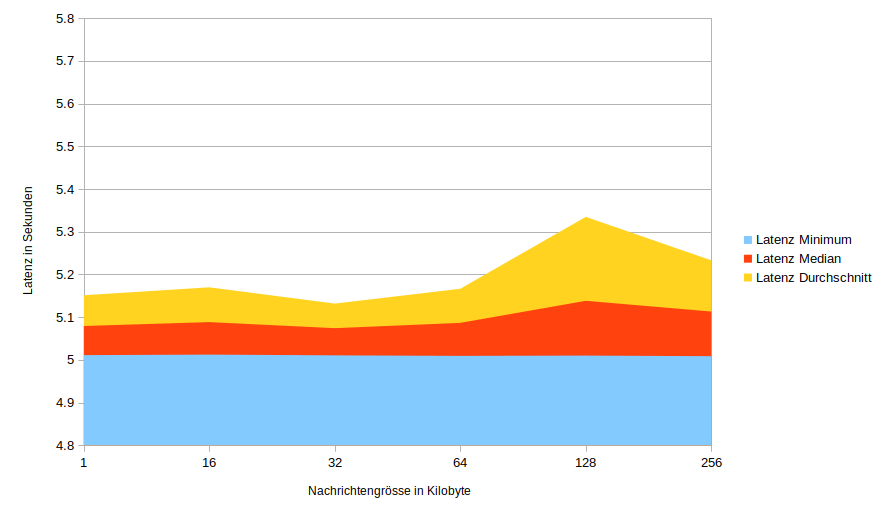
\includegraphics[width=1.1\textwidth]{img/auswertung-nachrichtengroesse.png}
  \caption{Nachrichtenlatenz bei verschiedener Nachrichtengrösse}\label{fig:auswertung-nachrichtengroesse}
\end{figure*}

Wie in der Grafik~\fullref{fig:auswertung-nachrichtengroesse} zu erkennen ist, verändert sich die Latenz abhängig von der Nachrichtengrösse nicht markant.
Ein kleiner Anstieg der Latenz ist jedoch ab der Nachrichtengrösse von 64 kB ersichtlich.
Jedoch macht dies keinen grossen Unterschied: Auch wenn die Nachrichtengrösse vervierfacht wird auf 256 kB, scheint das keinen grossen Einfluss auf die Latenz zu haben.
Es wurde in diesem Falle sogar eine tiefere Median- und Durchschnittslatenz gemessen, als mit einer Nachrichtengrösse von 128 kB.
Es wird vermutet, dass das an der Zwischenpuffergrösse liegt, welche bei I2P ebenfalls auf 64 kB gesetzt ist.

\section{Vergleich mit Anforderungen}\label{sec:vergleich_anforderungen}

Es wurde ein Stand der Technik ermittelt \seereq{SDTF} im Kapitel \fullref{ch:ideen_und_konzepte}, anhand dessen ein Konzept \seereq{TKON} erstellt und ein Teststand aufgebaut \seereq{TINF}.
Es wurde darauf geprüft, ob die Messungen reproduzierbar sind \seereq{TREP} im Abschnitt~\fullref{sec:validation_testumgebung}.
Es ist möglich, den Teststand und die Messungen zu konfigurieren, wie beschrieben im Abschnitt \fullref{sec:konfigurationsoptionen} \seereq{TCNF}.
Dabei kann man den Teststand auf bis zu 256 Knoten skalieren \seereq{TSCL},
wie beschrieben im Abschnitt \fullref{sec:scaling} und gezeigt bei der Messung im Abschnitt \fullref{sec:messung_nachrichtengroesse}.
Dabei ist das interne I2P-Netzwerk vom realen Testnetzwerk abgeschottet \seereq{TISO}, wie beschrieben im Abschnitt~\fullref{sec:netzwerkisolation}.
Optional hätten auch Tests im öffentlichen I2P-Netzwerk durchgeführt werden können \seereq{TNET}.
An verschiedenen Stellen im Programmcode wurde dies so vorgesehen, dass es in Zukunft möglich wäre.
Jedoch wird es nicht komplett unterstützt und wurde auch nie getestet.
Eine Messanlage zur Latenzmessung \seereq{TLAT} wurde entwickelt.
Es wurde die Möglichkeit implementiert die Bandbreite der einzelnen I2P-Knoten zu limitieren \seereq{TLIM}, jedoch wurde diese aus Zeitgründen nie komplett für Messungen eingesetzt; die anderen Experimente hatten Vorrang.
Es ist schnell möglich, ein neues Mess-Experiment zu starten \seereq{TVRS}: Man muss lediglich die Konfiguration anpassen und die Knoten erstellen.
Im besten Falle ist dies innerhalb von 5 Minuten möglich.
Soll jedoch etwas anderes als eine Latenzmessung durchgeführt werden, müsste die Messanlage angepasst werden.
Dies würde weiteren Entwicklungsaufwand mit sich bringen.
Die Evaluation und Auswertung der Messresultate \seereq{EVAL} wurde im Abschnitt \fullref{sec:messresultate} vorgenommen.
Die Ausführungszeiten der Tests wurden so gut wie möglich kurz gehalten \seereq{TPER}. Eine Messung mit 1000 Nachrichten dauert fast zwei Stunden, da die Nachrichten im Abstand von sechs Sekunden verschickt werden, um das Netzwerk nicht zu überlasten. Andere Experimente könnten hier eine bessere Test-Performance mit sich bringen.

Es wurde mit Kanban ein iteratives Projektmangement eingesetzt \seereq{ITER}.
Oft aber hatte man zu viel Overhead da ich zu genaue Meeting-Notizen für jedes kleine Meeting erstellt habe.
Zudem wurde als Bestandteil der Bachelorarbeit dieser Bericht erstellt \seereq{DOCS}, eine Zwischenpräsentation gehalten \seereq{PRES}, ein Web-Abstract erstellt \seereq{WEBA} und ein dazugehöriges Pitching-Video produziert \seereq{PVID}.
Somit konnten meisten Anforderungen erfüllt werden, inklusive den optionalen Anforderungen.

\section{Technische Aspekte}\label{sec:technische_aspekte}

Mit der Umstellung von der NixOS-basierten Lösung auf die auf Docker-compose-basierte Lösung ist
die Möglichkeit, I2P-Knoten auf mehrere Maschinen zu deployen, verloren gegangen.
Die Docker-Container werden mit Docker-compose so nur auf einem einzelnen Rechner erstellt, und
es können nicht ohne weiteres mehrere Testnetzwerke miteinander verbunden werden.
Mit diesem Ansatz kann nicht auf beliebig viele Knoten skaliert werden, da nur vertikal skaliert werden kann.
Dementsprechend ist dieser Ansatz durch existierende Hardware limitiert.

Für die Messanlage wurde ein eigener TCP-Server und TCP-Client in C implementiert, um genauere Messresultate zu erhalten.
Dies hat jedoch viel Zeit beansprucht und eine einfachere Lösung hätte
eventuell ähnlich genaue Resultate liefern können.
Die Auswertung der CSV-Dateien mit den Messresultaten mittels LibreOffice Calc (Excel-Pendant) war nicht unbedingt einfach und durchaus mühsam.
Vor allem war das Erstellen der Diagramme problematisch. Jedoch war dieses Vorgehen wohl aus Zeitgründen pragmatisch.

Zur Erstellung des Berichts und der Präsentation wurde die \LaTeX-Suite eingesetzt.
Dies hatte den Vorteil, dass stets in meinem Liebligseditor Vim gearbeitet werden konnte.
Zudem bietet \LaTe  mit BibiTeX eine Lösung zur Verwaltung von Quellen für ein Literaturverzeichnis und macht das Handhaben jedglicher Referenzen einfach. Weil es sich um reinen Text handelt, konnte auch die Versionsverwaltung Git für den Bericht eingesetzt werden.
Nachteil dieser Lösung ist jedoch, dass die Rechtschreibprüfung von Vim nicht so gut ist wie die Rechtschreibprüfung von Word.
Dies hat einen Mehraufwand verursacht.
Zudem musste oft im Internet nach passenden Befehlen und Paketen gesucht werden, um gewisse Teile des Berichts zu gestalten.
Jedoch konnte man einiges dazulernen und einen schön gestalteten Bericht abliefern.

\clearpage

\section{Vorgehen}\label{sec:eval_vorgehen}

Die verwendete Projektmangement-Methode Kanban war sicherlich hilfreich,
auch wenn man sich nicht immer strikt daran halten konnte.
Im Nachhinein hätte man sich den einen oder anderen Punkt mehr zu Herzen nehmen sollen,
zum Beispiel, dass man nicht gleichzeitig an mehreren Sachen hätte arbeiten sollen.
Oft hat man sich während der Entwicklung auch überstürzt und zu viele Änderungen auf einmal vorgenommen, sodass nicht mehr klar war, wieso etwas nun nicht mehr funktionierte.
Die wöchentlichen Meetings waren extrem hilfreich, den Kurs des Projektes zu steuern und schnell Feedback einzuholen.
Oft hat man sich im Detail verloren, sich zu viel vorgenommen oder überstürzt gehandelt.
Dies konnte durch die Meetings jeweils etwas reguliert werden.
Während die erstellten Meeting-Notizen hilfreich waren, haben sie aber auch oft zu viel Projektmanagement-Overhead geführt.

